\documentclass[10pt,border=3mm,tikz]{standalone}% better for developing drawings
\usepackage{tikz}
\usetikzlibrary{shapes.geometric, positioning, fit}% not needed

% not needed
\tikzset{mycylinder/.style={rectangle, shape border rotate=90, aspect=0.2, draw, fill=white, minimum width=2.5cm}}

% new
\tikzset{
    % ~~~ a server-pic with known dimensions ~~~~~~~~~~
    serv/.pic={
        \draw[fill=orange!30] (-1.2,-.3) rectangle (1.2,.3);% rectangle
        \draw[fill=orange!30] (-1.2,.3) -- (-.7,.9) -- (.7,.9) -- (1.2,.3) -- cycle;% trapezoid
        \draw[fill=white,draw=white] (.9,0) circle [radius=1mm];% knob with a white frame
        
        \foreach \i in {0, .3, .6, .9, 1.2}% some slits
            \draw[,draw=white,line width=1.6mm] (-1+\i,-.22) -- (-.8+\i,.22);
            % one slit; stroke is quite thick
    }
}

\begin{document}

 % ~~~ NEW ~~~~~~~~~~~~~
 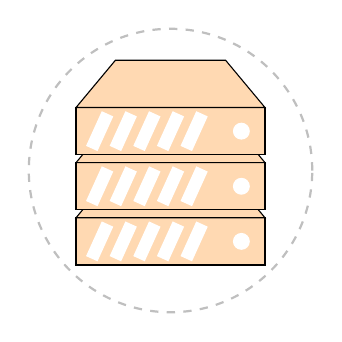
\begin{tikzpicture}
    % ~~~ putting some servers into known places ~~~~~
    \pic at (0,-.7) {serv};
    \pic at (0,  0) {serv}; % center server, but not center of total image
    \pic at (0,0.7) {serv};
    
    % ~~~ drawing the circle ~~~~~~~~~
    \draw [dashed,draw=gray!50, thick] (0,.2) circle [radius=18mm];% adjust y and r by iteration
 \end{tikzpicture}

% ~~~ current approach ~~~~~~~~~~
%\begin{figure}
%    \centering
    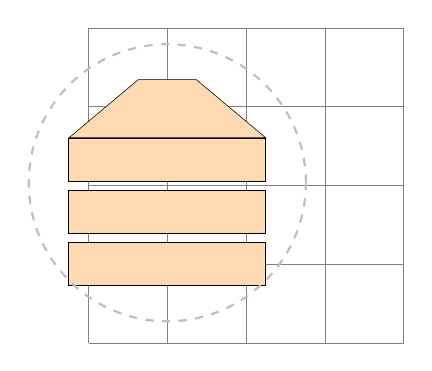
\begin{tikzpicture}[node distance=-4mm]
    \draw [help lines] (-1,-1) grid (3,3);
        \node[mycylinder, fill=orange!30] (C) {\phantom{Cloud Storage}};
        \node[mycylinder, above=of C,yshift=5mm, fill=orange!30] (A) {\phantom{Cloud Storage}};
        \node[mycylinder, above=of A,yshift=5mm, fill=orange!30] (B) {\phantom{Cloud Storage}};

        \node [trapezium, trapezium angle=40, minimum width=25mm, draw, thick,above=of B,fill=orange!30,yshift=4mm,line width=0.2pt] (T){};

        \node[draw, circle, dashed, inner sep=-1.2pt, draw=gray!50, thick, fit=(A)(B)(C)(T)] (D) {};
    \end{tikzpicture}
%\end{figure}
\end{document}